\documentclass[12pt]{article}
\usepackage[utf8]{inputenc}
\usepackage{graphicx}
\title{\textbf{Transformation of Random Variable\\}}
\author{M.Wahaj Tahir\\F191014@cfd.nu.edu.pk\\wahajt@acm.org}
\date{May 2022}
\usepackage{float}
\usepackage[export]{adjustbox}
\usepackage{blindtext}
\usepackage{indentfirst}

\begin{document}

\maketitle
\begin{figure}[b]
\centering
 
\includegraphics[scale=0.20]{Fast-Nuces.png}
\end{figure}
\clearpage

\large 
\clearpage
\begin{center}
\centering
    \textbf{To my mother who keeps on believing in me.}
\end{center}
    

\clearpage
\tableofcontents
\clearpage

\section{Abstract}
We consider transformations of random variables and derive the c.d.f. and density functions of the transformed random variables. A leading example is the probability integral transform, which transforms a random variable into a uniform random variable.A random variable is a numerical description of the outcome of a statistical experiment. It can be discrete or continuous depending upon the outcome of experiment.Often we are required to generate new distribution or density function with closed forms from a given
distribution. Programmatically, it might be easy, but sometimes looking beyond just numbers is
required to obtain specific parameters for new distributions such as mean, standard deviation, moment
generating functions, etc. Hence, knowing the methodology of generating new distribution by the
transformation of a random variable is significant. In this article, we will look at the transformation of
a random variable to create a new distribution from a continuous distribution given the transformation
function.
\clearpage

\section{Introduction}
\subsection{What is Transformation?}
Method of transformations (inverse mappings). Suppose we know the density function of $x$. Also suppose that the function $y =\phi(x)$ is differentiable and monotonic for values within its range for which the density $f(x) =0$.  This means that we can solve the equation $y =\phi(x)$  for x as a function of $y$.
\subsection{Methodology}
Consider a random variable $X$ with a PDF and CDF given by $f_X(x)$ and $F_X(x)$, respectively. Define a new random variable $Y$ such that $Y = g(X)$ for some function $g(·)$. What is the PDF, $f_Y(y)$ (or CDF), of the new random variable? This problem is often encountered in the study of systems where the PDF for the input random variable $X$ is known and the PDF for the output random variable Y needs to be determined. In such a case, we say that the input random variable has undergone a transformation.

Monotonically Increasing Functions To begin our exploration of transformations of random variables, let’s assume that the function is continuous, one-to-one, and monotonically increasing. A typical function of this form is illustrated in Figure 1. This assumption will be lifted later when we consider more general functions, but for now this simpler case applies. Under these assumptions, the inverse function, $X = g^{-1}(Y)$, exists and is well behaved. In order to obtain the PDF of Y, we first calculate the CDF. Recall that $FY(y) = Pr(Y ≤ y)$. Since there is a one-to-one relationship between values of $Y$ and their corresponding values of $X$, this CDF can be written in terms of $X$ according to
\begin{equation}
    F_Y(y)=Pr(g(X)\leq y)=Pr(X\leq g-1(y))=F_X(g^{-1}(y)).
\end{equation}
It can also be written as
\begin{equation}
    F_X(x)=F_Y(g(x))
\end{equation}

Differentiating Equation 1 with respect to y produces
\begin{equation}
 f_Y(y)=f_X(g^{-1}(y))\frac{{dg^{-1}(y)}}{dy}=f_X(x)\frac{dx}{dy}|_x_=_g_^{-1}(y)^{'}
\end{equation}

 Differentiating Equation 2 with respect to x produces
 \begin{equation}
  f_X(x)=f_Y(g(x))\frac{dy}{dx}\Rightarrow f_Y(y)=\frac{f_X(x)}{dy} |_x_=_g_^{-1}(y)
\end{equation}
\begin{figure}
    \centering
    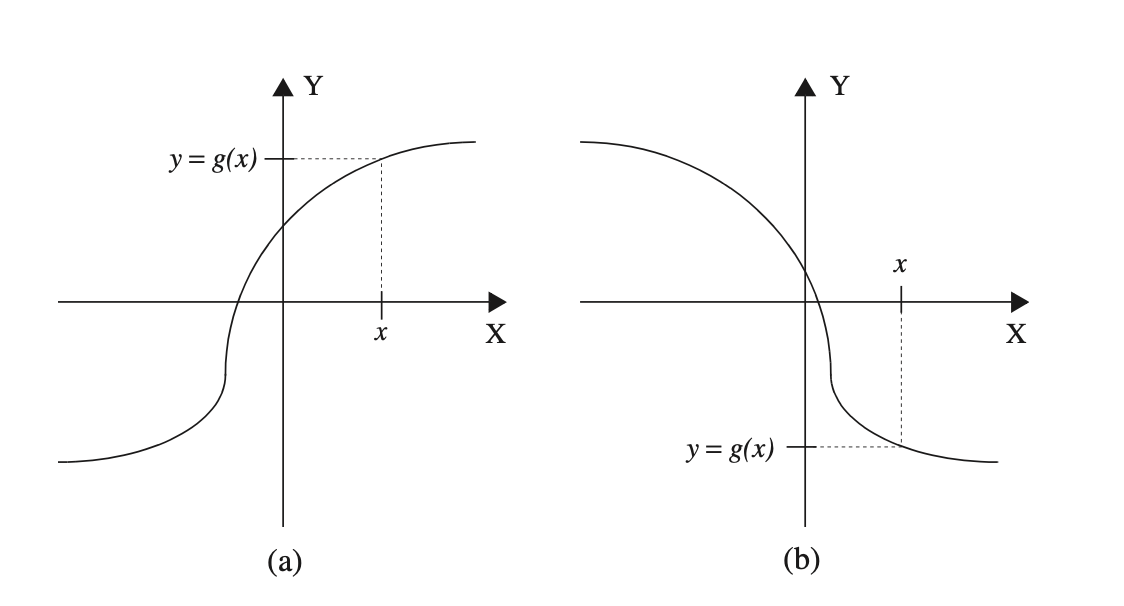
\includegraphics[scale=0.60]{Graphy.png}
    \caption{A monotonic increasing function (a) and a monotonic decreasing function (b).}
    \label{fig:my_label}
\end{figure}
\subsection{Non-monotonic Functions}
Non-monotonic Functions Finally, we consider a general function that is not necessarily monotonic. Figure 2 illustrates one such example. In this case, we cannot associate the event {$Y \leq y$} with events of the form {$X \leq g^{−1}(y)$} or {$X \geq g^{−1}(y)$} because the transformation is not monotonic. To avoid this problem, we calculate the PDF of $Y$ directly, rather than first finding the CDF. Consider an event of the form $y \leq Y < y + dy$ for an infinitesimal $dy$. The probability of this event is {$Pr(y \leq Y < y + dy) = f_Y(y)dy$}. In order to relate the PDF of Y to the PDF of X, we relate the event ${y \leq Y < y + dy}$ to events involving the random variable $X$. Because the transformation is not monotonic, there may be several values of $x$ that map to the same value of $y$. These are the roots of the equation $x = g^{-1}(y)$. Let us refer to these roots as $x_1, x_2, . . . , x_N$ . Furthermore, let $X^{+}$ be the subset of these roots at which the function $g(x)$ has a positive slope, and similarly let  $X^{-}$ be the remaining roots for which the slope of the function is negative.
\begin{figure}[t]
    \centering
    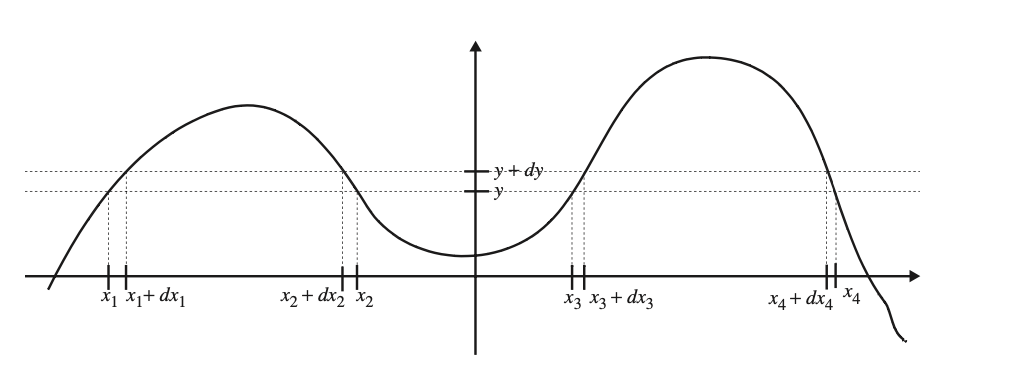
\includegraphics[scale=0.80]{Nonmontonic.png}
    \caption{Non-monotonic Function}
    \label{fig:my_label}
\end{figure}
This graphic represents the same property of Non-monotonic Functions.


\clearpage
\section{Application of Random Variable}
Probability plays a vital role in our life that we couldn’t even predict, Simply I would say we can predict the future or moreover  we can predict qiyammat (just a  joke), By the probability, we can predict car accidents ratio in one month, Cancer detection, Earthquakes, Weather Conditions, Time of the body start decomposing and many more, Today’s world is living in technology there are different domains of Computer Sciences where the probability plays its role are
\begin{enumerate}
    \item 
    Machine learning
     \item 
    Data Science
     \item 
     Artificial Intelligence
      \item 
     Simulation of system 
\end{enumerate}

  

\clearpage
\section{References}
My References 
\cite{lu2017structural}
\cite{tong2021normal}
\cite{zhao2018complete}
\cite{zhao2020monotonic}
\cite{zhao2021orthogonal}
\cite{chambers1976method}
\bibliographystyle{plain}
\bibliography{Mybib}


\end{document}
